\documentclass[10pt]{beamer}
\usepackage{uglibeamer2}
\title{Parcours de graphes}
\author{NSI2}
%NOT_VISITED = (.5, .5, .5)
%CURRENT = (1, 0, 0)
%WAITING = (.5, 0, .5)
%VISITED = (.5, .5, 1)

\definecolor{graphbleu}{rgb}{.5, .5, 1}
\definecolor{graphrouge}{rgb}{1, 0,0}
\definecolor{graphviolet}{rgb}{.5, 0,0.5}
\definecolor{graphautre}{rgb}{.5,.5,.5}

\begin{document}
\maketitle

\begin{frame}{Orientés ou non orientés ?}
On peut considérer des graphes orientés ou non. Cela ne change pas grand chose au principe :
\begin{enumerate}[--]
	\item dans le cas d'un graphe non orienté, on parcourt un graphe de voisins en voisins;
    \item si le graphe est orienté on le parcourt de successeurs en successeurs.
\end{enumerate}
\end{frame}

\section*{Parcours en profondeur}
\begin{frame}{Principe du parcours en profondeur}
À partir d'un sommet de départ, on va chercher à aller:
\begin{enumerate}
	\item le plus « loin» possible d'abord.
    \item dans toutes les directions.
\end{enumerate}
Le parcours en profondeur est appelé \textit{Depth First Search} ou DFS en anglais.
\end{frame}
\begin{frame}{Multiplicité des parcours}
\'Etant donné un graphe et un sommet de départ, il n'y a pas en général qu'un seul parcours en profondeur qui commence par ce sommet car l'ordre dans lequel on choisit chaque voisin d'un
sommet est \textit{a priori} arbitraire.
\end{frame}
\begin{frame}{Implémentation itérative}
On peut implémenter un parcours DFS de manière itérative en utilisant une \alert{pile} dans laquelle on empile les prochains sommets à traiter (voisins du sommet en cours).\\
Il faut cependant faire attention à ne pas empiler plusieurs fois un sommet, c'est pourquoi on crée une liste des sommets non empilés.
\end{frame}

\begin{frame}{Exemple}
\begin{enumerate}[--]
    \item \color{graphautre} sommet non visité non empilé
	\item \color{graphviolet} voisin non visité mais empilé
    \item \color{graphrouge} sommet en cours de visite
    \item \color{graphbleu} sommet déjà visité
\end{enumerate}

\only<1>{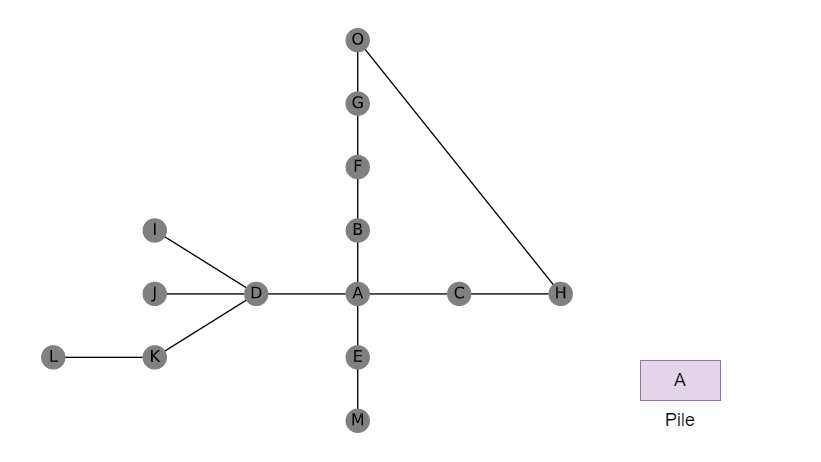
\includegraphics[width=\linewidth]{img/dfs/00.png}}
\only<2>{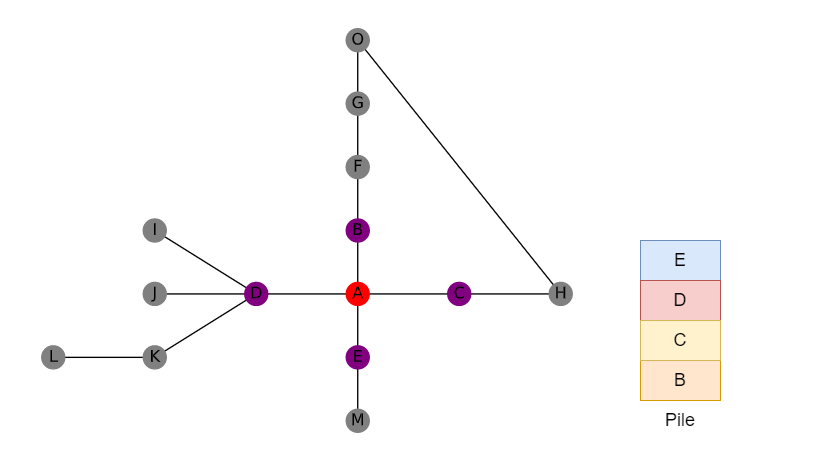
\includegraphics[width=\linewidth]{img/dfs/01.png}}
\only<3>{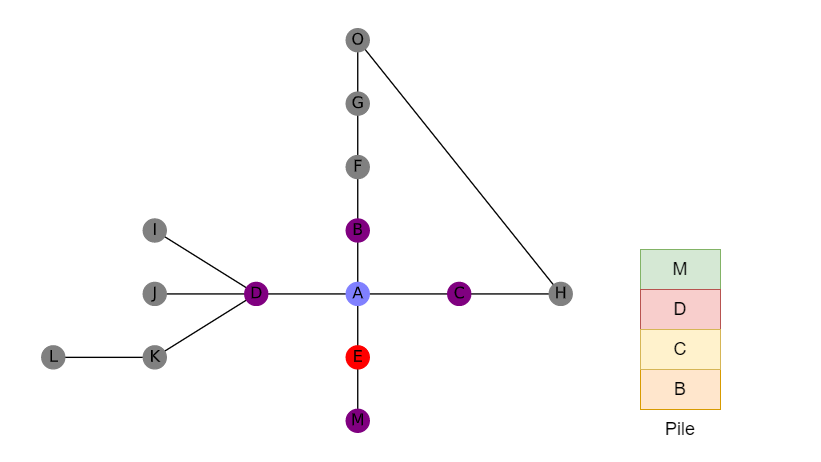
\includegraphics[width=\linewidth]{img/dfs/02.png}}
\only<4>{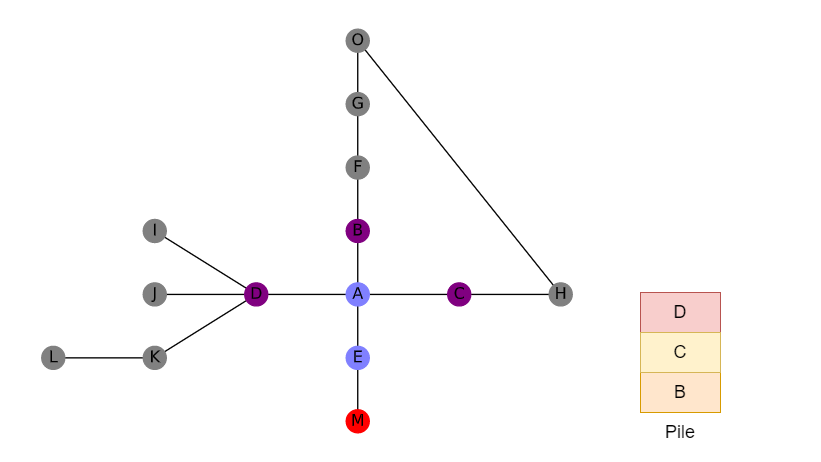
\includegraphics[width=\linewidth]{img/dfs/03.png}}
\only<5>{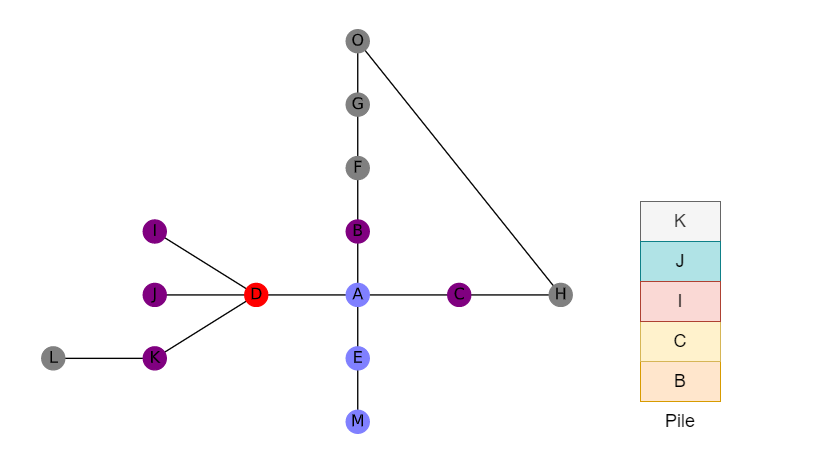
\includegraphics[width=\linewidth]{img/dfs/04.png}}
\only<6>{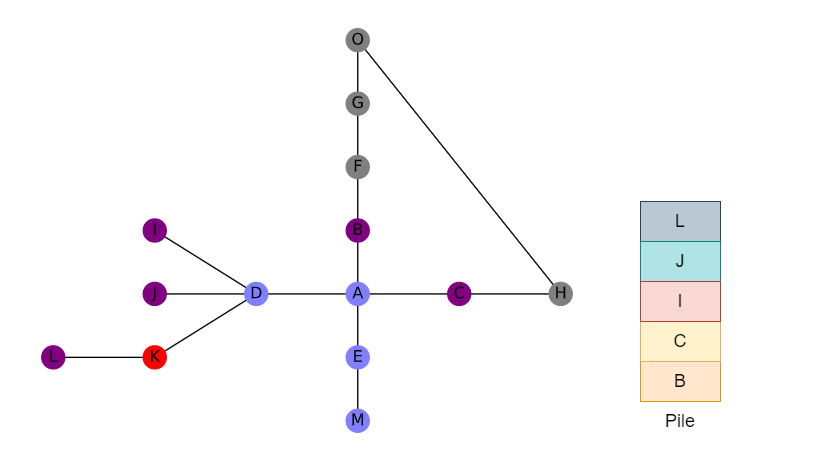
\includegraphics[width=\linewidth]{img/dfs/05.png}}
\only<7>{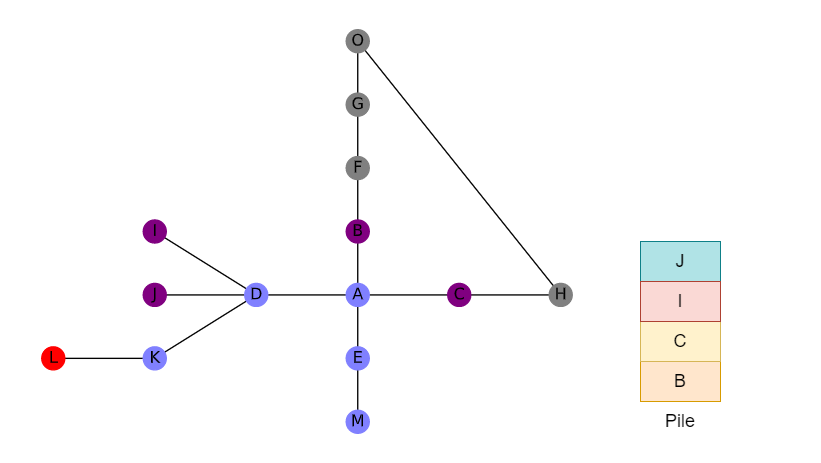
\includegraphics[width=\linewidth]{img/dfs/06.png}}
\only<8>{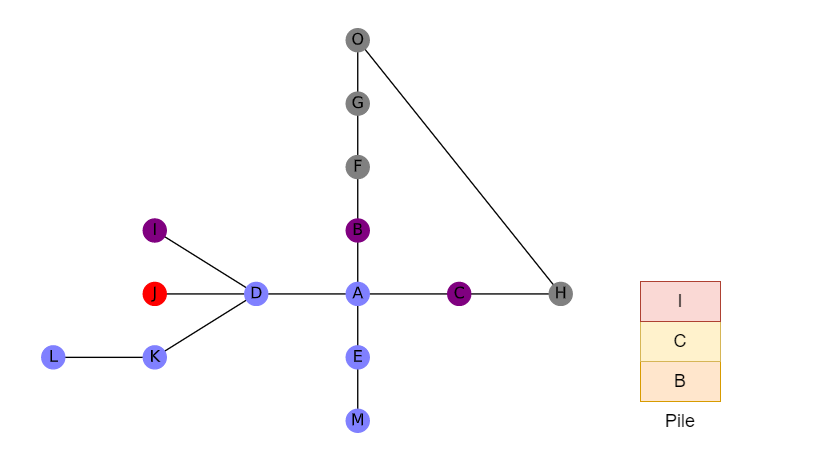
\includegraphics[width=\linewidth]{img/dfs/07.png}}
\only<9>{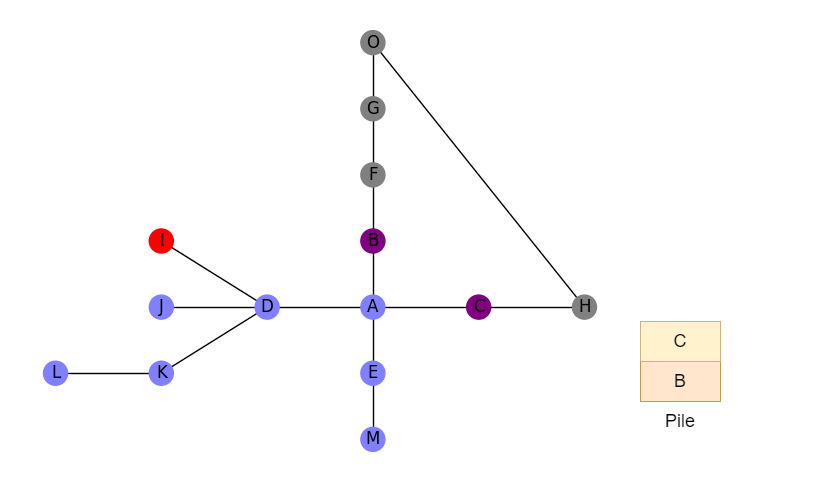
\includegraphics[width=\linewidth]{img/dfs/08.png}}
\only<10>{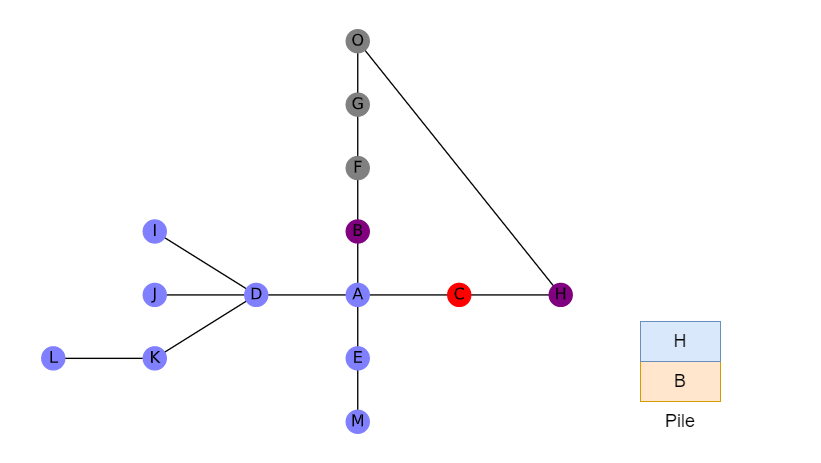
\includegraphics[width=\linewidth]{img/dfs/09.png}}
\only<11>{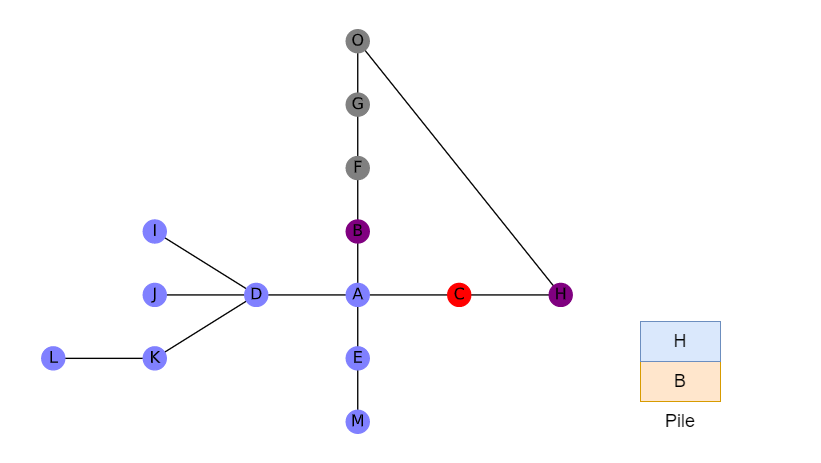
\includegraphics[width=\linewidth]{img/dfs/10.png}}
\only<12>{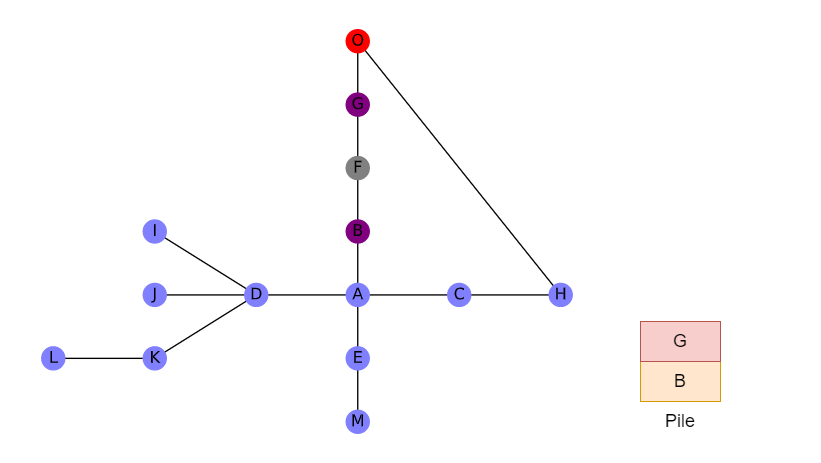
\includegraphics[width=\linewidth]{img/dfs/11.png}}
\only<13>{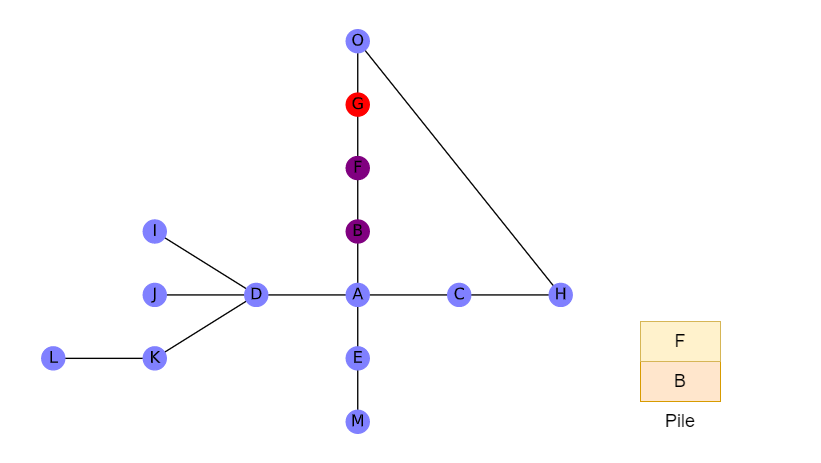
\includegraphics[width=\linewidth]{img/dfs/12.png}}
\only<14>{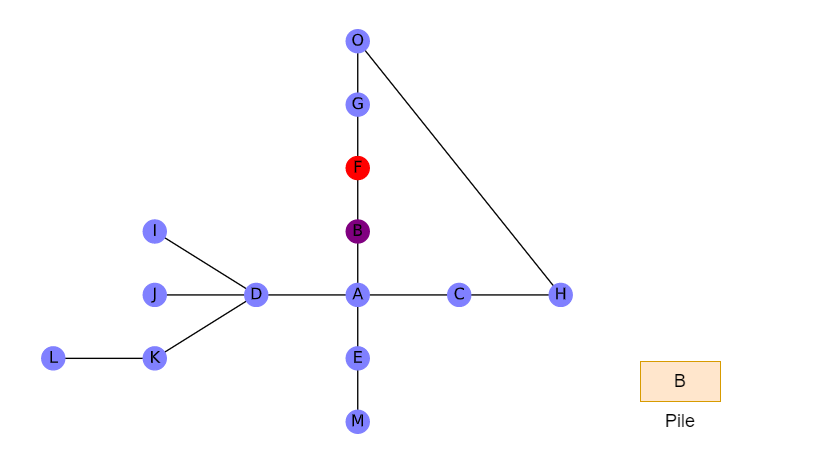
\includegraphics[width=\linewidth]{img/dfs/13.png}}
\only<15>{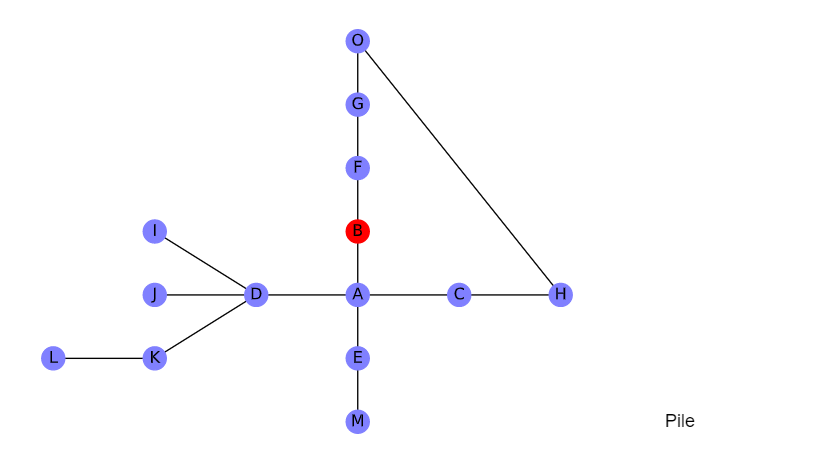
\includegraphics[width=\linewidth]{img/dfs/14.png}}

\end{frame}

\begin{frame}[fragile]{Implémentation itérative}
\small
\begin{verbatim}
fonction dfs( G : graphe, d : départ ) -> liste
    variables
        p : pile
        sommets_restants, parcours : liste
    début
        sommets_restants = sommets_de_G
        empiler d sur p
        retirer d de sommets_restants
        tant que p n'est pas vide :
            s = dépiler de p
            ajouter s à parcours
            pour chaque voisin v de s :
                si v est dans sommets_restants :
                    empiler v sur p
                    retirer v de sommets_restants
        renvoyer pacours
    fin
\end{verbatim}
\normalsize
\end{frame}


\begin{frame}{Remarque}
On peut également implémenter le parcours DFS de manière récursive.
\end{frame}
\section*{Parcours en largeur}
\begin{frame}{Principe du parcours en largeur}
À partir d'un sommet de départ, on va chercher à visiter
\begin{enumerate}
	\item tous les voisins directs d'abord, dans toutes les « directions» possibles.
    \item puis les voisins des voisins et ainsi de suite le plus loin possible.
\end{enumerate}
Le parcours en largeur est appelé \textit{Breadth First Search} ou BFS en anglais.
\end{frame}
\begin{frame}{Remarque}
Tout comme DFS, BFS dépend de l'ordre dans lequel on va parcourir les sommets voisins, il n'y a donc pas (en général) unicité du parcours en largeur partant d'un sommet donné.
\end{frame}

\begin{frame}{Implémentation itérative}
On peut implémenter un parcours BFS de manière identique à DFS, à ceci près qu'on utilise une \alert{file} à la place de la pile.
\end{frame}

\begin{frame}[fragile]{Implémentation itérative}
    \small
\begin{verbatim}
fonction bfs( G : graphe, d : départ ) -> liste
    variables
        f : file
        sommets_restants, parcours : liste
    début
        sommets_restants = sommets_de_G
        enfiler d dans f
        retirer d de sommets_restants
        tant que f n'est pas vide :
            s = défiler de f
            ajouter s à parcours
            pour chaque voisin v de s :
                si v est dans sommets_restants :
                    enfiler v dans f
                    retirer v de sommets_restants
        renvoyer pacours
    fin
\end{verbatim}
\normalsize
\end{frame}

\begin{frame}{Exemple}
\only<1>{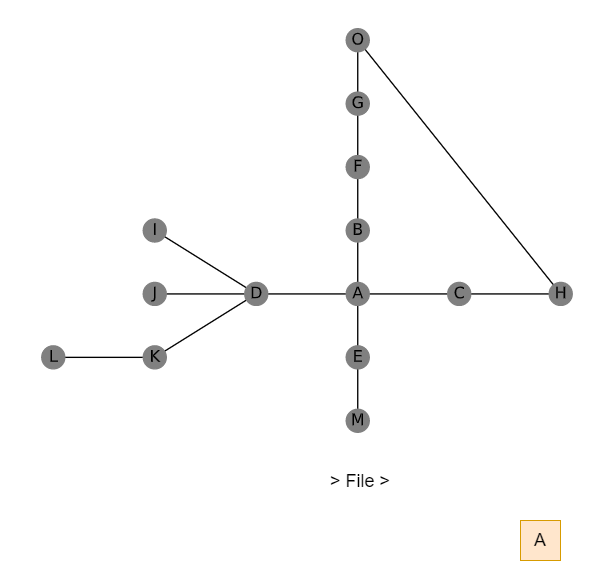
\includegraphics[width=8cm]{img/bfs/00.png}}
\only<2>{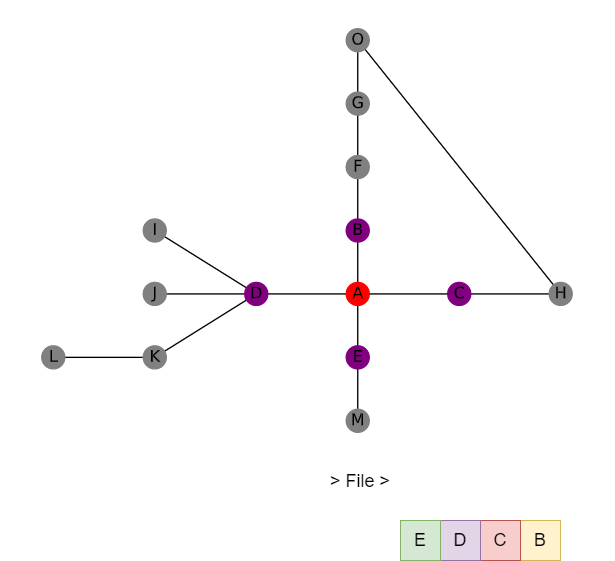
\includegraphics[width=8cm]{img/bfs/01.png}}
\only<3>{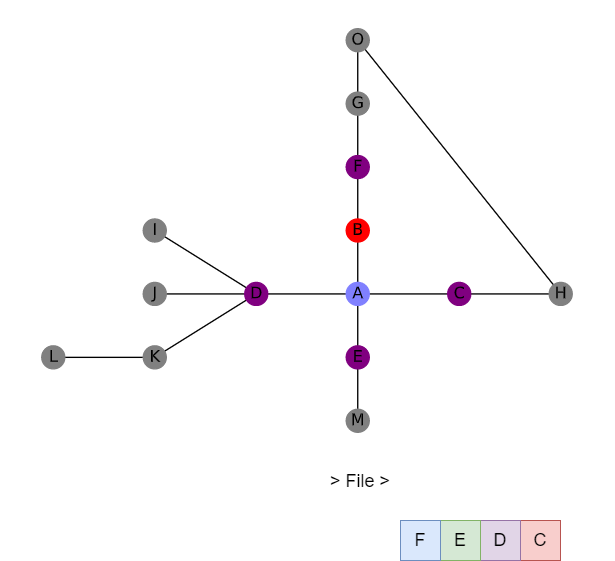
\includegraphics[width=8cm]{img/bfs/02.png}}
\only<4>{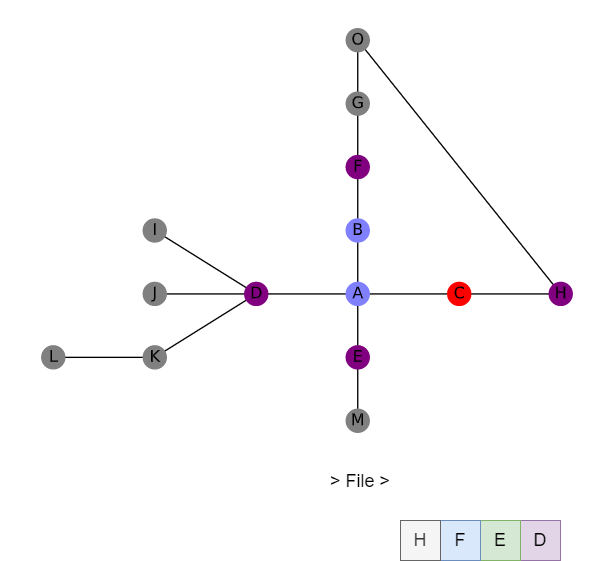
\includegraphics[width=8cm]{img/bfs/03.png}}
\only<5>{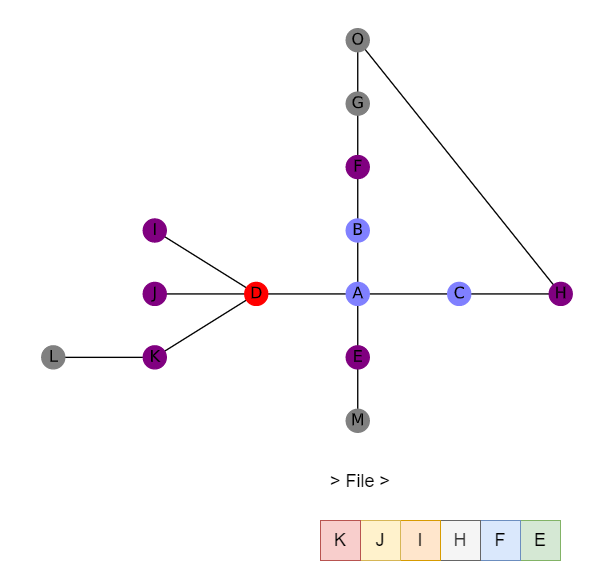
\includegraphics[width=8cm]{img/bfs/04.png}}
\only<6>{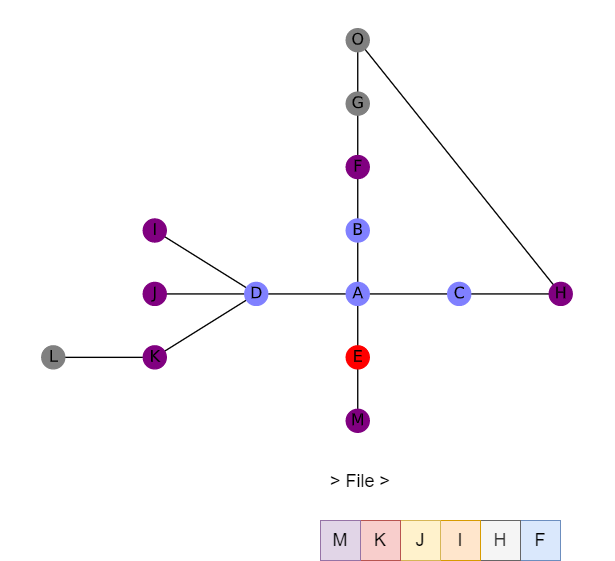
\includegraphics[width=8cm]{img/bfs/05.png}}
\only<7>{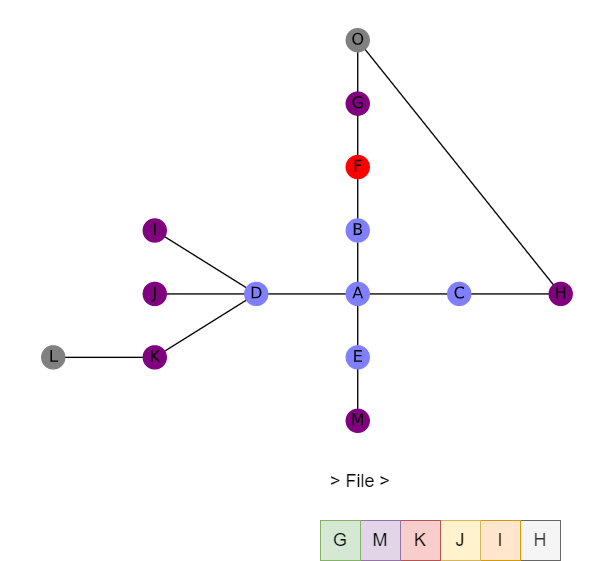
\includegraphics[width=8cm]{img/bfs/06.png}}
\only<8>{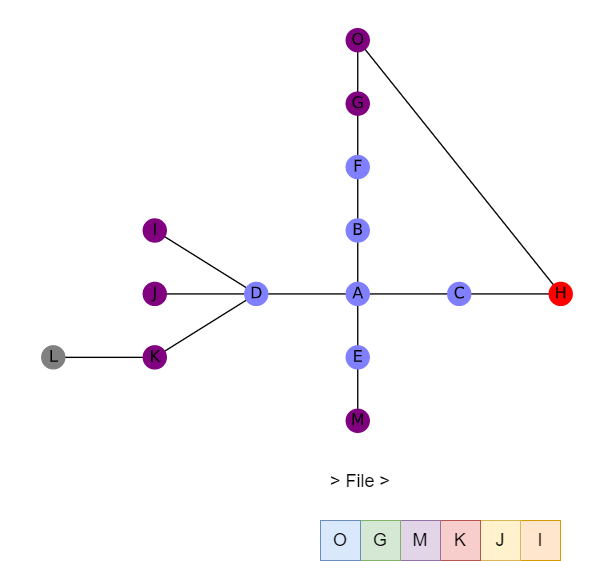
\includegraphics[width=8cm]{img/bfs/07.png}}
\only<9>{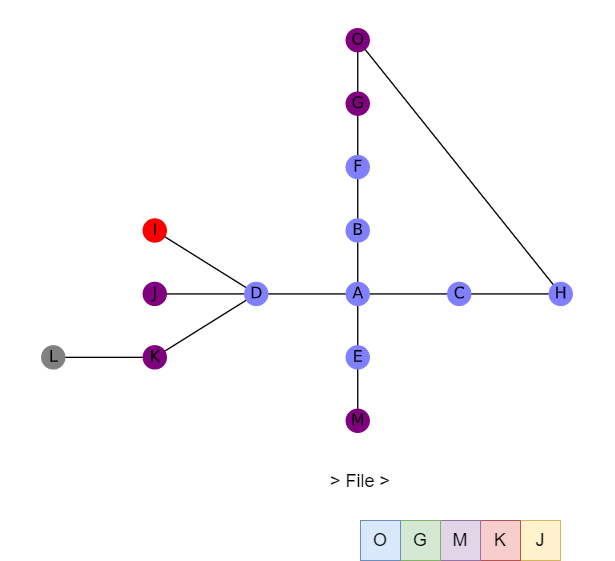
\includegraphics[width=8cm]{img/bfs/08.png}}
\only<10>{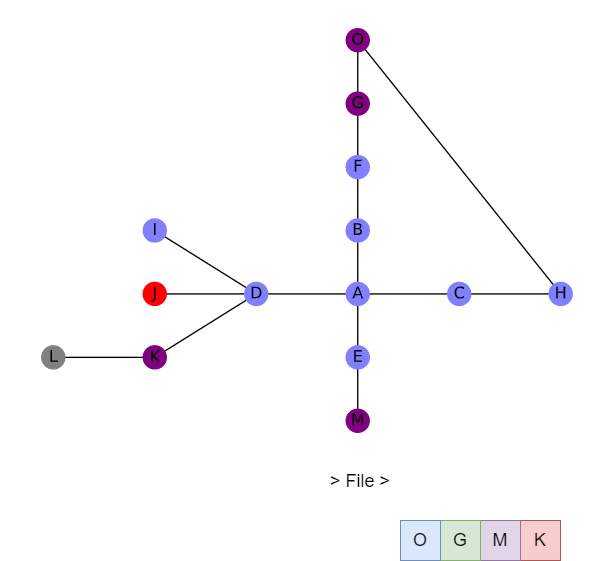
\includegraphics[width=8cm]{img/bfs/09.png}}
\only<11>{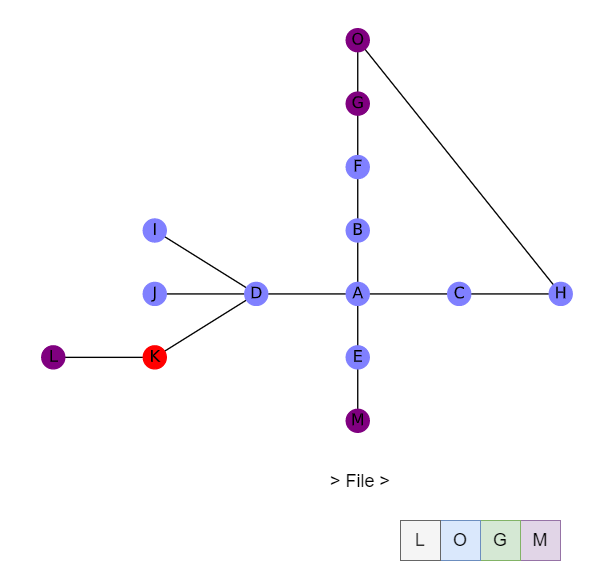
\includegraphics[width=8cm]{img/bfs/10.png}}
\only<12>{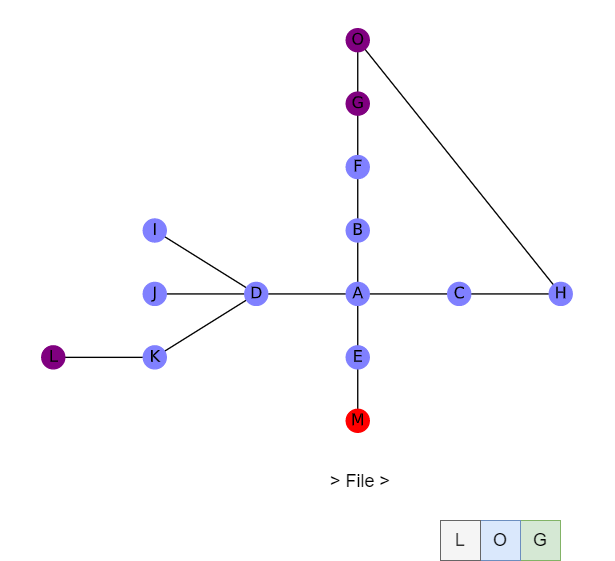
\includegraphics[width=8cm]{img/bfs/11.png}}
\only<13>{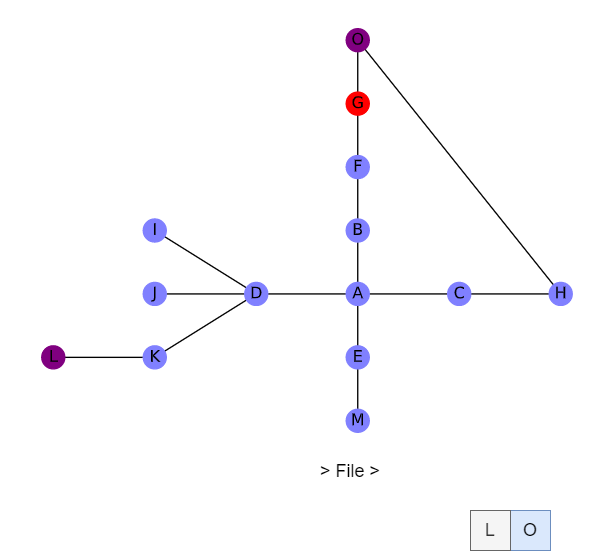
\includegraphics[width=8cm]{img/bfs/12.png}}
\only<14>{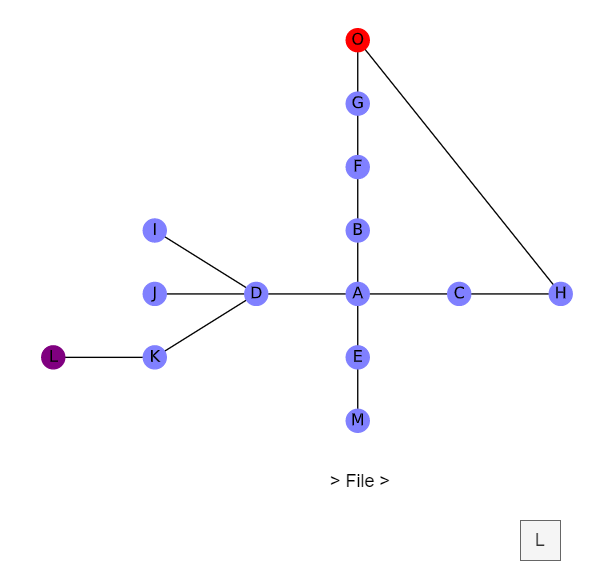
\includegraphics[width=8cm]{img/bfs/13.png}}
\only<15>{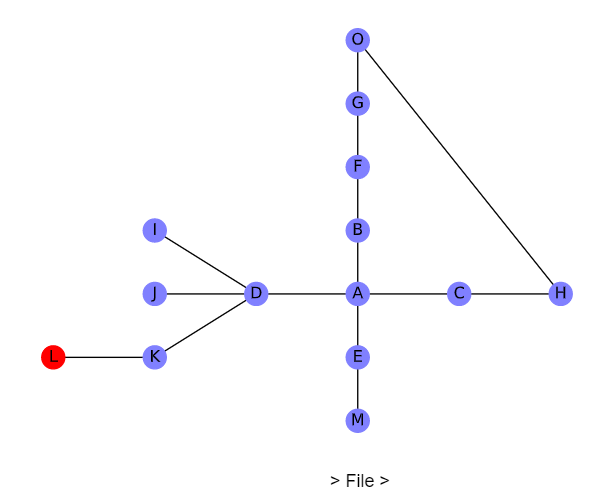
\includegraphics[width=8cm]{img/bfs/14.png}}
\end{frame}

\end{document}